\documentclass{article}
\usepackage{latexsym}
\usepackage[a4paper]{geometry}
\usepackage{fullpage}
\usepackage{hyperref}
\usepackage{amsmath}
\usepackage{xcolor}
\usepackage{booktabs}
\usepackage{graphicx}
\usepackage{tikz}
\usepackage[export]{adjustbox}
\usepackage{comment}
\usepackage[style=iso]{datetime2}
%\usetikzlibrary{calc}
\usetikzlibrary{arrows,positioning} 
\tikzset{
    %Define style for course boxes
    courseboxv/.style={
           rectangle,
           draw=blue!50!black, very thick,
           fill=blue!10,
           minimum height=8cm,
           minimum width=4cm,
           text width=3.9cm,
           text centered,
           font=\bfseries\sffamily},
    courseboxh/.style={
           courseboxv,
           minimum height=4cm,
           minimum width=8cm,
           text width=7.9cm},
    courseboxhh/.style={
           courseboxh,
           minimum height=4cm,
           minimum width=16cm,
           text width=15.9cm}
}
\def\frameseparation{1.5cm}
\def\scalingfactor{.9}

\newcommand{\secref}[1]{Section~\ref{sec:#1}}
\newcommand{\secreff}[2]{Sections \ref{sec:#1} and \ref{sec:#2}}
\newcommand{\eqnref}[1]{Equation~\eqref{eq:#1}}
\newcommand{\eqnreff}[2]{Equations \eqref{eq:#1} and \eqref{eq:#2}}
\newcommand{\eqnrefff}[3]{Equations \eqref{eq:#1}, \eqref{eq:#2} and \eqref{eq:#3}}
\newcommand{\figref}[1]{Figure \ref{fig:#1}} 
\newcommand{\figreff}[2]{Figures \ref{fig:#1} and \ref{fig:#2}}
\newcommand{\figrefff}[3]{Figures \ref{fig:#1}, \ref{fig:#2} and \ref{fig:#3}}
\newcommand{\tabref}[1]{Table~\ref{tab:#1}}
\newcommand{\tabreff}[2]{Tables~\ref{tab:#1} and \ref{tab:#2}}
\newcommand{\tabrefff}[3]{Tables~\ref{tab:#1}, \ref{tab:#2} and \ref{tab:#3}}

\def\year{2025--2026}
\title{EITA66 Design of Systems for Digital Transformation\\\year}
%\title{EITA65 Digitalisering -- realisering och systemdesign med användarperspektiv\\\year}
\author{{\huge Sensors with Sense HAT}\\\\Raspberry Pi Project -- Part 2}
%\\Version \DTMnow}
%\date{}

\begin{document}
\newgeometry{left=2.5cm,right=2.5cm,bottom=1.5cm}% for placing course schematic lower on first page
\clearpage\maketitle
\thispagestyle{empty}% to remove page numbering on first page

\begin{itemize}
\item 
\includegraphics[width=3mm]{person.png} This project will be done individually, but you will work \textit{together} in groups of 3 or 4.
\item You will not get detailed step-by-step instructions. Figuring out how to reach the goal is part of the project. (being a collaborative doer)
\item The results of this project part will be used in the next so document, and backup, your work.
\end{itemize}

\vspace{.1cm}
\begin{center}
\begin{tabular}{l}
\toprule[1.5pt]
\parbox{0.8\linewidth}{
\vspace{.2cm}{\Large Learning goals:}
\begin{itemize}
\item Getting hands-on experience with sensors.
\item Getting acquainted with Python.
\item Practicing collaboration skills.
\end{itemize}}\\
\bottomrule[1.5pt]
\end{tabular}
\end{center}

\vfill
\begin{center}
\includegraphics[width=100mm]{sense_hat_no_bg.png}
\end{center}
\vspace{2cm}

\begin{comment}
\begin{center}
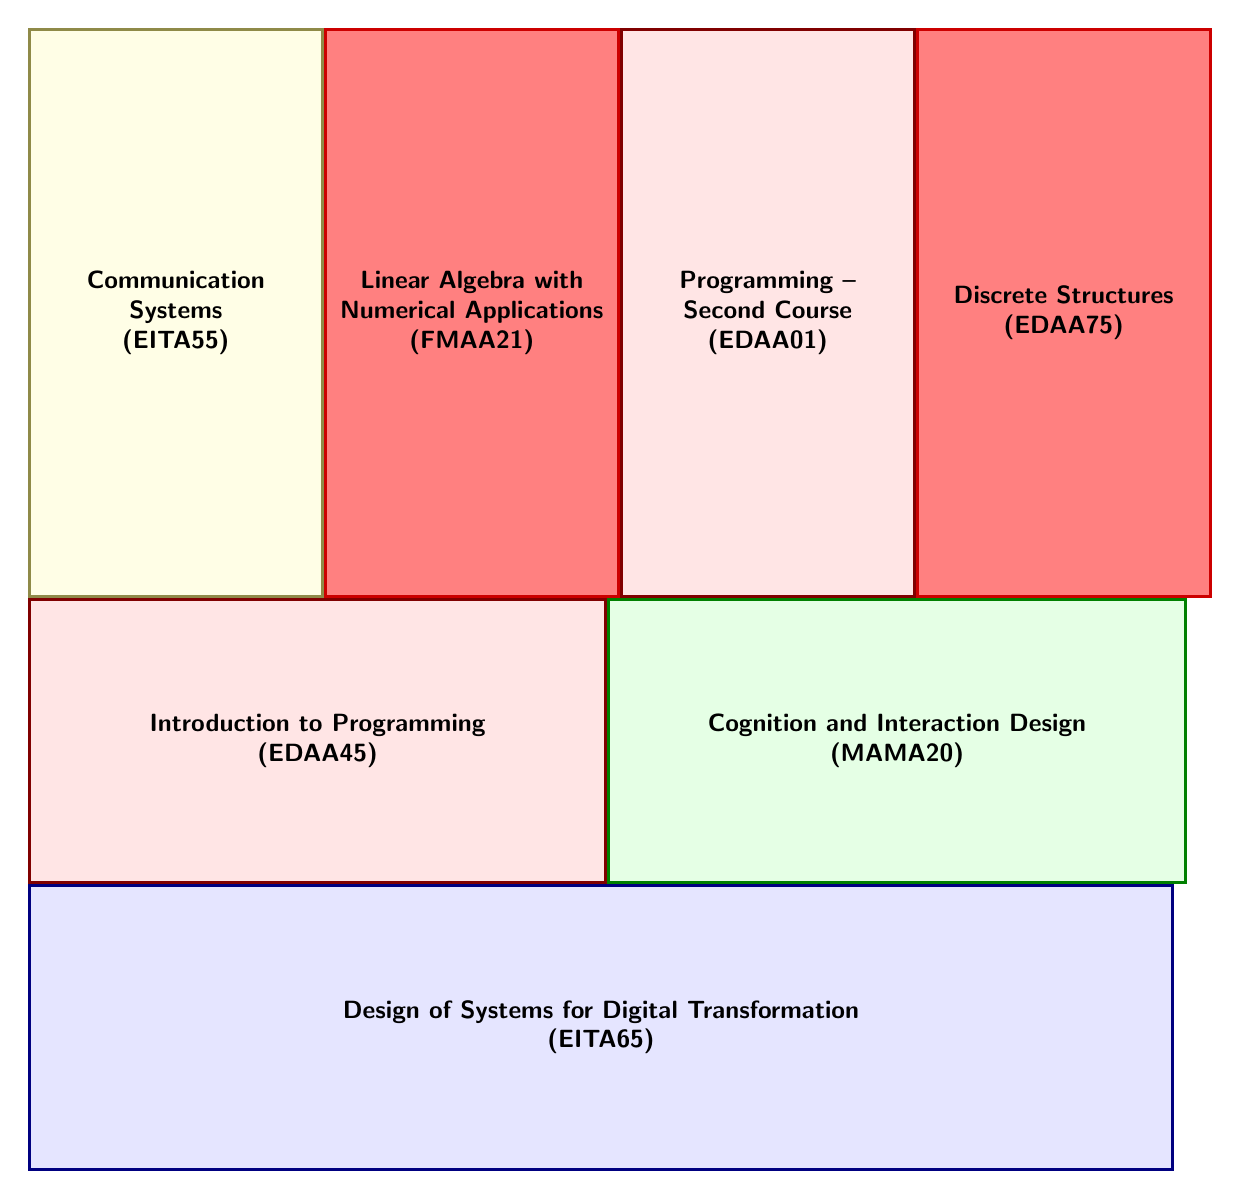
\begin{tikzpicture}[>=latex, node distance=0cm,scale=\scalingfactor,every node/.style={scale=\scalingfactor}]
\node[courseboxv, draw=yellow!50!black, fill=yellow!10] (EITA55) {Communication Systems\\(EITA55)};
\node[courseboxv, draw=red!80!black, fill=red!50, anchor=west] (FMAA21) at (EITA55.east){Linear Algebra with Numerical Applications\\(FMAA21)};
\node[courseboxv, draw=red!50!black, fill=red!10, anchor=west] (EDAA01) at (FMAA21.east){Programming -- Second Course\\(EDAA01)};
\node[courseboxv, draw=red!80!black, fill=red!50, anchor=west] (EDAA75) at (EDAA01.east){Discrete Structures\\(EDAA75)};
%\node[courseboxh, preaction={clip, postaction={fill=red!10, draw=red!50!black, line width=2mm}}, anchor=north west] (EDAA45) at (EITA55.south west){Introduction to Programming\\(EDAA45)};
\node[courseboxh, draw=red!50!black, fill=red!10, anchor=north west] (EDAA45) at (EITA55.south west){Introduction to Programming\\(EDAA45)};
%\node[courseboxh, draw=green!50!black, fill=green!10, anchor=west] (MAMA20) at (EDAA45.east){Cognition and Interaction Design\\(MAMA20)};
\node[courseboxh, draw=green!50!black, fill=green!10, right=of EDAA45] (MAMA20) {Cognition and Interaction Design\\(MAMA20)};
\node[courseboxhh, anchor=north west] (EITA65) at (EDAA45.south west){Design of Systems for Digital Transformation\\(EITA65)};
%\node[anchor=south east, inner sep=2pt, font=\bfseries\sffamily\scriptsize] at (EDA625.south east) {Helsingborg};
%\path[->,draw=black,dotted,thick] (EIT060.east) -- (EITF05.west);
%\path[->,draw=black,dotted,thick] (EIT060.south) -- (EITN50.north);
%\path[->,draw=black,dotted,thick] (EITF05.south) -- (EITN41.north);
%\draw[draw=blue!50!black, very thick] ($(EIT060.north west)+(-\frameseparation,\frameseparation)$) rectangle ($(EDA625.south east)+(\frameseparation,-\frameseparation)$);
\end{tikzpicture}
\end{center}
\end{comment}

\restoregeometry
\newpage


\section{Introduction}
\noindent In this project part you will get acquainted with sensors and the Python programming language.

\noindent In this part of the project you will
\begin{itemize}
\item[1.] learn about sensors,
\item[2.] code using Python,
\item[3.] use the sense HAT for the first time.
\end{itemize}

\section{What are sensors?}
Sensors are somethings that gives you information about your surroundings. In the human body our sensors are our senses (duh): vision, sound, touch, smell and taste. Smartphones also have sensors, but theirs are a camera, an accelerometer (detects if you tilt your phone), a gyroscope (orientation details and direction) and a magnetometer (tells you where north is) \cite{foss}. In the Sense HAT that you have there are seven different sensors;
\begin{itemize}
    \item Gyroscope,
    \item Accelerometer,
    \item Magnetometer,
    \item Temperature,
    \item Barometric pressure,
    \item Humidity,
    \item Joystick.
\end{itemize}
You can think of a joystick as a directional pressure sensor.
% \section{GPIO}
% The GPIO are the metallic pins sticking up from your Pi. GPIO is short for \emph{General-Purpose Input/Output} and are used to communicate with something outside of the Pi, like a small motor or LEDs. In figure \ref{fig:gpio} you can see what the different pins are used for. Some provides electricity and most of them are used for communication \cite{gpio}. Read more about GPIOs at {\color{blue}\href{https://en.wikipedia.org/wiki/General-purpose_input/output}{Wikipedia}} and {\color{blue}\href{https://projects.raspberrypi.org/en/projects/physical-computing/1}{Raspberry Pis website}}. 
% \begin{figure}[h]
%     \centering
%     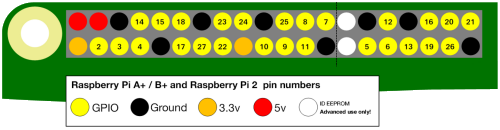
\includegraphics[width=140mm]{pinout.png}
%     \caption{The setup of the GPIOs on the Pi}
%     \label{fig:gpio}
% \end{figure}

\section{Python}
In this project you will use Python. Python is a popular programming language used around the world, and is a good first programming language to start with since it has a simple and very readable code syntax. Let's try to code!

\subsection{Using a Python IDE}
An Integrated Development Environment (IDE) is a graphical user interface (GUI) that aims to make programming easier.
\begin{itemize}
    \item[1.] Start Thonny Python IDE (found in the Programming tab in the menu -- click on the raspberry in the upper left of the screen).
    \item[2.] Write \texttt{print("Hello Pi!")} in the \textless untitled\textgreater  section.
    \item[3.] Save the code you have written to a file named \verb!my_code.py!. For now it is good enough to save all your Python-files in the same directory.
    \item[4.] Run the code! Hopefully you will see \texttt{Hello Pi!} in the shell in the lower part of the window.
\end{itemize}
How does that work under the hood? The Thonny Python IDE first takes the Python code you have written and feeds it into a special program -- a Python interpreter. The interpreter then reads the code and does what the code tells it to do (it interprets the code). Then, the output (what is printed) is handed back to the Thonny Python IDE, which displays the result in the lower part of the window.
Simply put, the Thonny Python IDE is a graphical interface to using a Python program.

\subsection{Using the Terminal}
You can, of course, take the more hard-core approach of running the Python program yourself. It is quite simple, this is how you do it:
\begin{itemize}
    \item[1.] Start a Terminal (click on the Terminal icon in the top left of the screen).
    \item[2.] If necessary, navigate to the folder where you placed \verb!my_code.py!.
    \item[3.] Run the Python program and pass your file name as input as
    \begin{equation}
    \label{eq:run_code}
    \verb!python my_code.py!
    \end{equation}
    and press \verb!ENTER!. The output text \texttt{Hello Pi!} should now appear in the Terminal.
\end{itemize}
The current version of Raspberry Pi OS (Trixie) comes with version 3 of Python installed only. Therefore, the \verb!python! command will use that version. You can explicitly state that you want to use Python version 3 when you run your program:
\begin{equation}
\verb!python3 my_code.py!
\end{equation}
The result will, however, be the same. To check which specific version number(s) your Python programs have, use
\begin{equation}
\verb!python --version!
\end{equation}
and
\begin{equation}
\verb!python3 --version!
\end{equation}
respectively.

\subsection{Printing and looping}
Recalling that you will not learn the entire Python language, but rather use Python as a convenient tool, what is most useful to you at the moment is printing values and control loops.\\

\noindent Change your program as follows.
    \item[1.] Open your program file \verb!my_code.py! in Thonny or in a text editor.
    \item[2.] Change the file content to
\begin{center}
    \verb!for x in range(6):!\\
    \verb!  print(x)        !
\end{center}    
    \item[3.] Save and run your code using the Terminal command you used earlier \eqref{eq:run_code}.
\end{itemize}
What is the output? Try changing the code to
\begin{center}
    \verb!for x in range(2,6):!\\
    \verb!  print(x)          !
\end{center}
What is the output this time?\\

\noindent Sometimes infinite loops are useful as well.
You can write one as follows.
\begin{center}
    \verb!x = 0      !\\
    \verb! while True:!\\
    \verb!  x += 1   !\\
    \verb!  print(x) !
\end{center}
Use the command
\begin{equation}
\label{eq:ctrlc}
\verb!Ctrl + C   !
\end{equation}
when you want to stop your program from running.

\newpage
\noindent To get acquainted with formatting output text, modify the code as follows and then run the code, stopping the execution using command \eqref{eq:ctrlc} once more.
\begin{center}
    \verb!x = 0                                    !\\
    \verb!print(f"The number {x} is large,")       !\\
    \verb!while True:                              !\\
    \verb!  x += 1                                 !\\
    \verb!   print(f"and the number {x} is larger,")!\\
\end{center}
You are now ready to move on to the next section :)

\section{The Sense HAT}
The acronym HAT means \emph{Hardware Attached on Top} and is often used for Raspberry Pi's different hardware extensions. One such extension is the Sense HAT. To learn how to use your HAT, follow the {\color{blue}\href{https://projects.raspberrypi.org/en/projects/getting-started-with-the-sense-hat/0}{tutorial (\texttt{https://projects.raspberrypi.org/en/projects/getting-started-with-the-sense-hat/0})}} on\\ how to sense the world around you with it as well as display messages on the LEDs. The goal is to be able to use the matrix of LEDs, get a reading from each different Sense HAT sensor and to print data from them. As for coding in Python, you should be able to look at and run existing code, and modify the code you have been given. Please don't get stuck on a particular assignment since it is not the main goal for you to create Python code.\\

\noindent {\bf Note 1: }\parbox[t]{14cm}{When you use the Sense Hat you might get a warning saying that the TCS34725 colour sensor cannot be initialised. This is normal and due to that the version of the Sense Hat you are using (version 1) does not have such a sensor. We will not use the colour sensor in the course so this is not a problem. You can just ignore it.}

\noindent {\bf Note 2: }\parbox[t]{14cm}{Some Raspberries have trouble recognising the Sense HAT and display an error message saying ''OSERROR: Cannot detect RPi-Sense FB device'' when you try to access it. If this happens do the following (you only need to do this once):\\1. Open a Terminal window and give the following command:\\\texttt{sudo nano /boot/firmware/config.txt}\\2. A text editor starts in the terminal window. Go to the end of the file and add the line:\\\texttt{dtoverlay=rpi\_sense}\\3. Save the file and exit by pressing \texttt{Ctrl+X} followed by \texttt{Y} and finally press ENTER.\\4. Reboot your Raspberry.}

\section{Lab Goal}
{\textcolor{red}{The task of this lab is to write a Python program that detects the joystick movement and shows a corresponding arrow of the same direction on the LED display. Show the TAs your result when you finish the task. The joystick examples together with the last {\color{blue}{\href{https://projects.raspberrypi.org/en/projects/getting-started-with-the-sense-hat/10}{challenge}}} in the given instruction can help you on your way.}

%Please stop the tutorial when you have reached the \emph{Using the joystick} section.

% \section{The Ultrasound Sensor}
% The sensor that looks like Wall-E's eyes is an ultrasound sensor. It is used to measure the distance from an obstacle in front of it. To attach it to the Raspberry Pi, you will need to use the breadboard two resistors and at least 5 wires to connect. In {\color{blue}\href{https://tutorials-raspberrypi.com/raspberry-pi-ultrasonic-sensor-hc-sr04/}{this website}} you will find a clear guide on how to connect the wires, as well as a sample Python script that measures distances with the ultra-sonic sensor.\\

% \noindent{\bf Note 1: }\parbox[t]{14cm}{The resistors that you have been given are \texttt{1 kOhm} and \texttt{2 kOhm}. Replace the 470 Ohm resistor with the 2 kOhm and the 330 Ohm resistor with the 1 kOhm. But how do you know which one is which? Go to {\color{blue}\href{https://resistorcolorcodecalc.com/}{this website}} and find out. As a hint I can tell you that the first band on one is red, and the other one brown.}\\

% \vspace{0.3cm}

% \noindent{\bf Note 2: }\parbox[t]{14cm}{You have more GPIOs than in the tutorial, but the ones that are being used are the most left ones in figure \ref{fig:gpio}. If you compare the schematics you can see that they are the same.}\\

% \vspace{0.1cm}

% \noindent{\bf Note 3: }\parbox[t]{14cm}{You have to be a bit creative when attaching your wires since you only have female-male wires. But you'll be fine.}\\

% \vspace{0.1cm}

% \noindent{\bf Note 4: }\parbox[t]{14cm}{If you use different GIPOs for \emph{Trig} and \emph{Echo} on the ultrasonic sensor instead of the ones provided in the example, remember to change the PIN numbers in the script before you run it. }\\

% \begin{center}
% 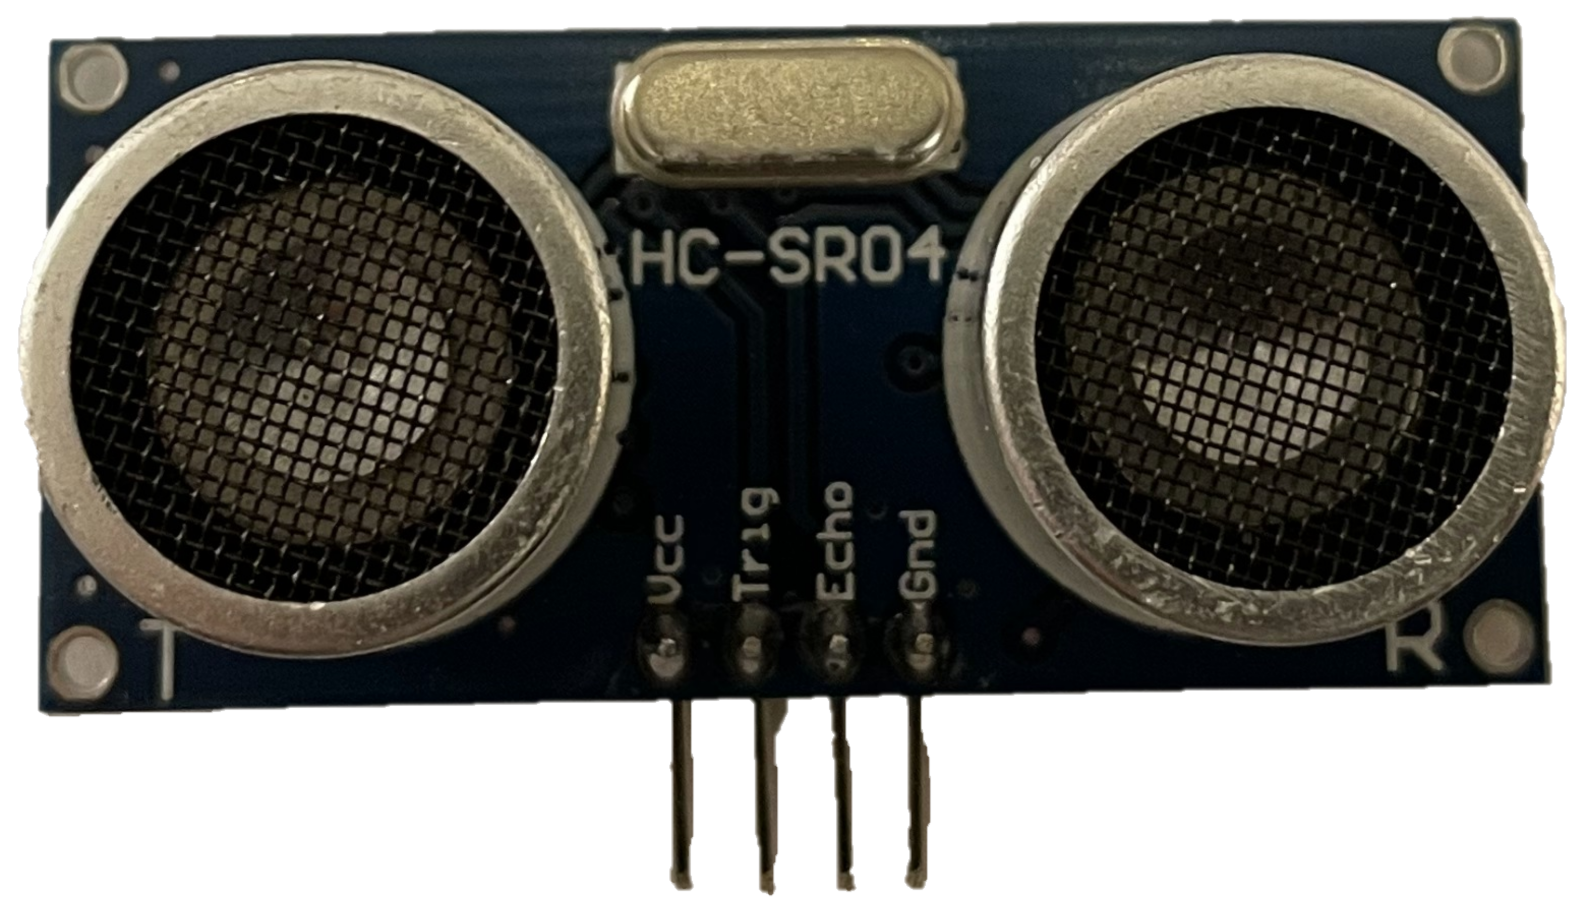
\includegraphics[width=80mm]{sensor_ultrasound_no_bg.png}
% \end{center}
% %how to connect
% %how to interact with it


%\section{Helpful Hints}
%{\bf Hint 1: }\parbox[t]{14cm}{Open up a terminal using the command \texttt{Ctrl + Alt + T}}\\
%{\bf Hint 2: }\parbox[t]{14cm}{Using the joystick as a sensor and storing directions as \textit{North}, \textit{South}, %\textit{East} or \textit{West} or something similar can be useful for the drone project.}\\
\vspace{1cm}
\begin{center}
\huge Good luck!
\end{center}

\begin{thebibliography}{10}
\bibliographystyle{plain}
% \bibitem{iso-date-time} ISO 8601 -- Date and Time Format, \url{https://www.iso.org/iso-8601-date-and-time-format.html}, last accessed on 2021-09-21.
\bibitem{foss} FOSSBYTES -- Which Sensors Do I Have In My Smartphone?, \url{https://fossbytes.com/which-smartphone-sensors-how-work/}, last accessed on 2025-10-30.
% \bibitem{gpio} GPIO pins, \url{https://projects.raspberrypi.org/en/projects/physical-computing/1}, last accessed on 2021-09-21.
\end{thebibliography}
\end{document}
